\documentclass{beamer}

\mode<presentation>
{
  \usetheme{Darmstadt}
  \usecolortheme{beaver}
  \usefonttheme{serif}
  \setbeamertemplate{navigation symbols}{}
  \setbeamertemplate{caption}[numbered]
}

\usepackage[english]{babel}
\usepackage[utf8]{inputenc}
\usepackage{booktabs}
\usepackage{amsmath}
\usepackage{graphicx}
\graphicspath{{figs/}}

\title[Multi-Task ViT]{Multi-Task Learning with Vision Transformers:\\Joint Classification and Saliency Prediction}
\author{Nicholas Welsh}
\institute{Florida Institute of Technology\\Department of Computer Science \& Mathematics}
\date{March 2026}

\begin{document}

\begin{frame}
  \titlepage
\end{frame}

\begin{frame}{Outline}
  \tableofcontents
\end{frame}

% ============================================================
\section{Motivation}
% ============================================================

\begin{frame}{Why Multi-Task Learning?}
\begin{itemize}
  \item Most deep learning models do one thing at a time: classify, detect, or segment.
  \item Humans solve many visual tasks simultaneously using shared representations.
  \item \textbf{Multi-task learning} trains one model on multiple tasks, encouraging a shared backbone to learn features useful for each.
  \item Potential benefits: better generalization, more efficient use of data and compute.
\end{itemize}
\vfill
\textbf{Our question:} Can a single Vision Transformer classify images \emph{and} predict where humans look?
\end{frame}

\begin{frame}{Why Saliency?}
\begin{itemize}
  \item \textbf{Saliency prediction} estimates where people look when viewing an image.
  \item Related to classification: object recognition and visual attention share low-level features (edges, textures, object boundaries).
  \item The SALICON dataset provides dense fixation maps for COCO images, enabling supervised training.
  \item Pairing classification labels with saliency ground truth lets us study how the two tasks interact inside a shared model.
\end{itemize}
\end{frame}

% ============================================================
\section{Model}
% ============================================================

\begin{frame}{Vision Transformer (DeiT-Small)}
\begin{itemize}
  \item \textbf{DeiT-Small}: a data-efficient Vision Transformer pretrained on ImageNet.
  \item Splits each $224 \times 224$ image into a grid of $16 \times 16$ patches $\rightarrow$ 196 patch tokens + 1 CLS token.
  \item 12 transformer layers, 384-dimensional embeddings, 22M parameters.
  \item We fine-tune the entire backbone on our paired dataset.
\end{itemize}
\end{frame}

\begin{frame}{Multi-Task Architecture}
\begin{center}
  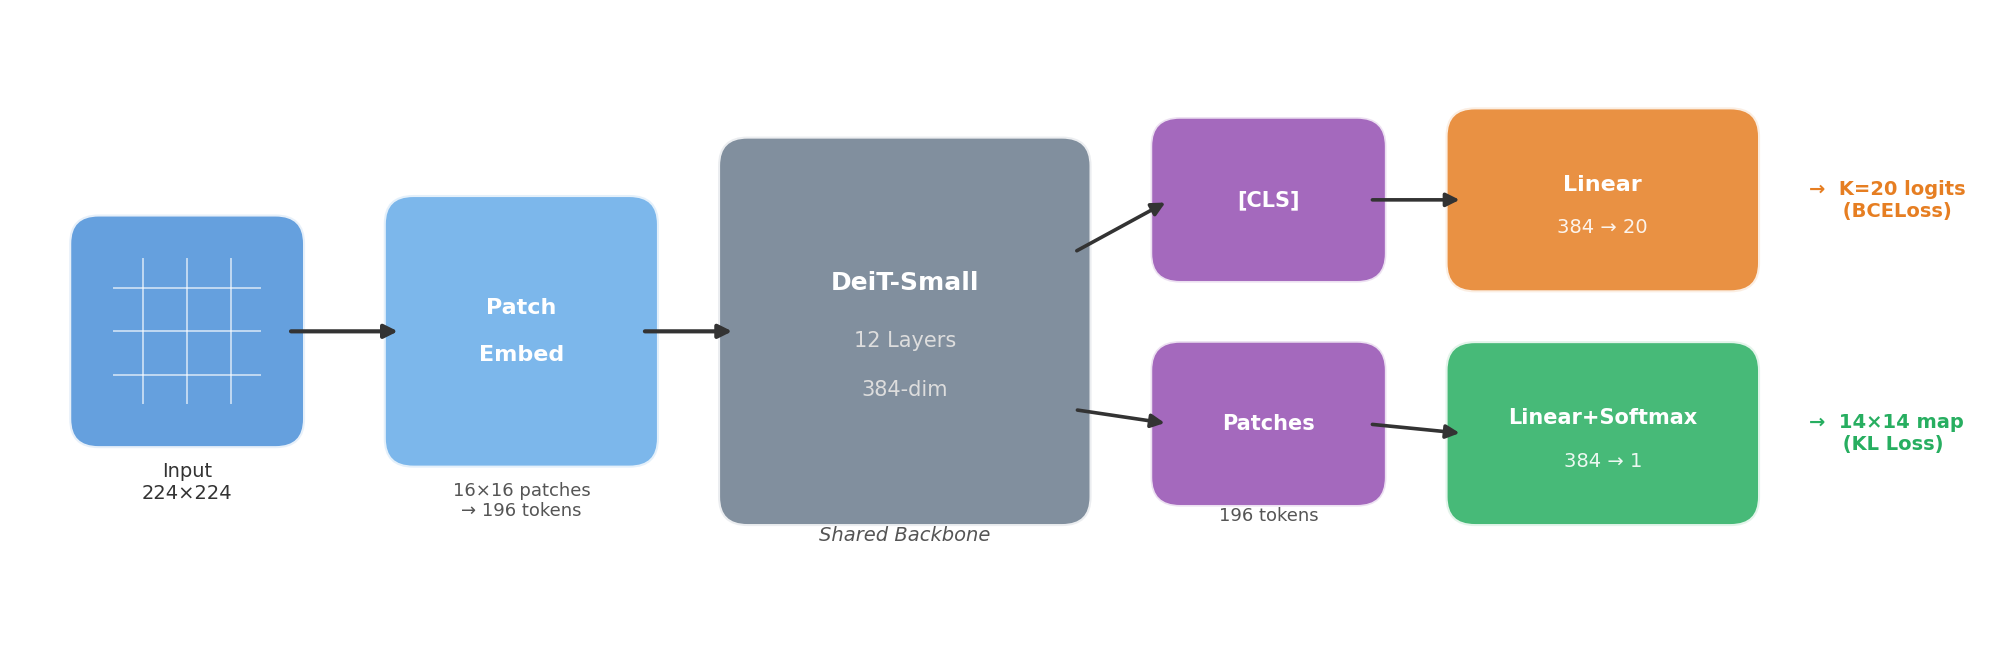
\includegraphics[width=0.85\linewidth]{../../../runs/figures/architecture.png}
\end{center}
\begin{itemize}
  \item \textbf{Classification head:} Linear layer on CLS token $\rightarrow$ 20 category logits.
  \item \textbf{Saliency head:} Linear layer on each patch token $\rightarrow$ softmax $\rightarrow$ $14\!\times\!14$ probability distribution.
\end{itemize}
\end{frame}

\begin{frame}{Why This Design?}
\begin{itemize}
  \item The CLS token aggregates global information (good for classification).
  \item Patch tokens retain spatial information (good for saliency).
  \item Both heads share the same backbone, so features learned for one task can help the other.
  \item The softmax on the saliency head ensures valid probability distributions by construction, which pairs naturally with KL divergence loss.
\end{itemize}
\end{frame}

% ============================================================
\section{Data}
% ============================================================

\begin{frame}{Datasets}
\begin{columns}
\column{0.55\textwidth}
\begin{itemize}
  \item \textbf{SALICON}: fixation density maps for 10,000 train / 5,000 val COCO images.
  \item Collected via mouse-contingent gaze tracking (approximates eye tracking at scale).
  \item \textbf{COCO 2014}: bounding-box annotations for 80 object categories.
  \item We select the top 20 most frequent categories and create binary label vectors.
\end{itemize}
\column{0.45\textwidth}
\begin{center}
  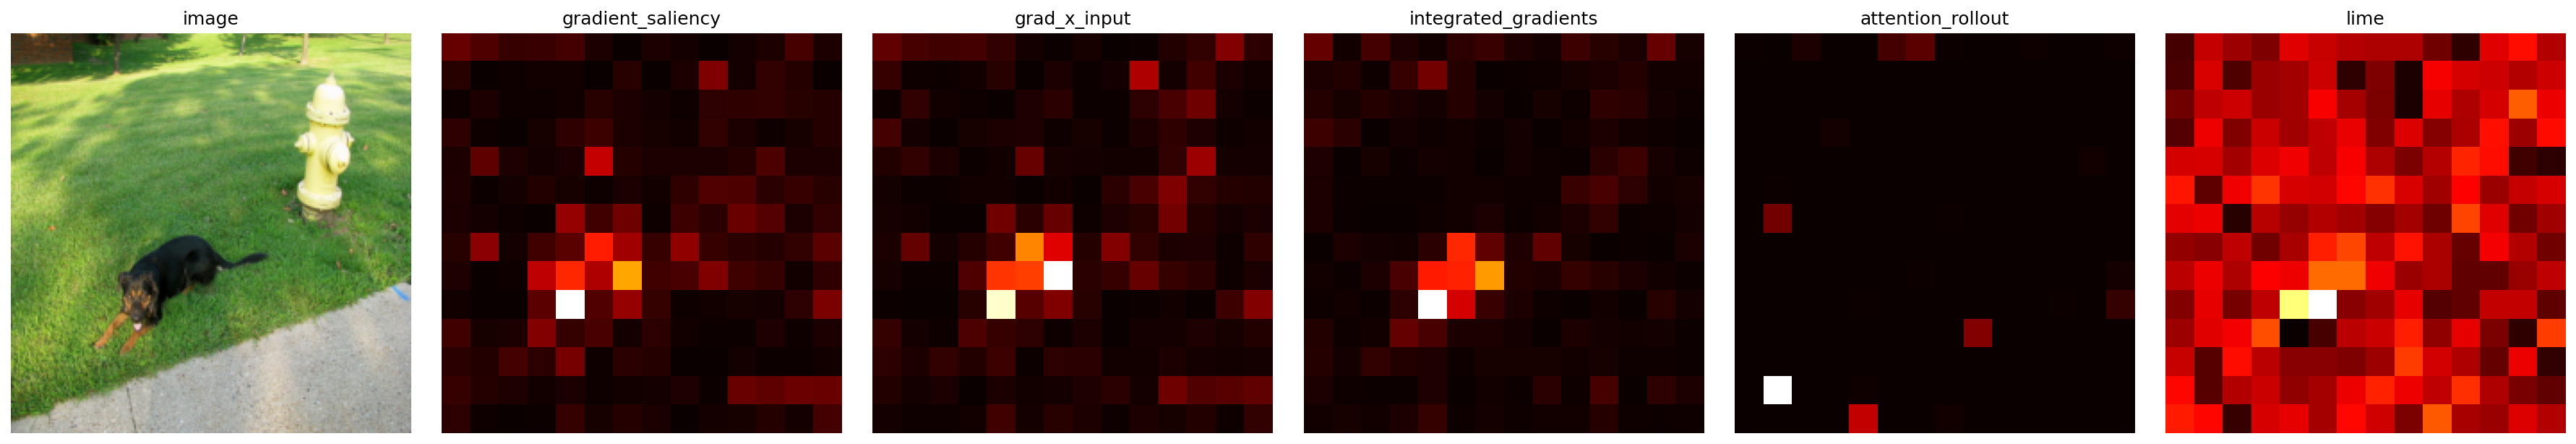
\includegraphics[width=\linewidth]{report_comparison_323.png}
\end{center}
\small Example: image with ground-truth saliency overlay and XAI attributions.
\end{columns}
\end{frame}

\begin{frame}{Preprocessing}
\begin{itemize}
  \item Images resized to $224 \times 224$, normalized with ImageNet statistics.
  \item No spatial augmentations (would need identical transforms on saliency maps).
  \item Saliency maps processed at two resolutions:
  \begin{itemize}
    \item $224 \times 224$ (full resolution, for visualization)
    \item $14 \times 14$ (patch grid, for training and evaluation)
  \end{itemize}
  \item Grid-resolution maps normalized to sum to 1 (probability distribution over patches).
\end{itemize}
\end{frame}

% ============================================================
\section{Experiment}
% ============================================================

\begin{frame}{Training Setup}
\begin{itemize}
  \item \textbf{Optimizer:} AdamW, lr = $10^{-4}$, weight decay = $10^{-4}$
  \item \textbf{Schedule:} cosine annealing over 15 epochs
  \item \textbf{Batch size:} 32
  \item \textbf{Loss:} $\mathcal{L} = \mathcal{L}_{\text{cls}} + \lambda \cdot \mathcal{L}_{\text{sal}}$ with $\lambda = 1.0$
  \begin{itemize}
    \item Classification: binary cross-entropy with logits
    \item Saliency: KL divergence (or MSE for ablation)
  \end{itemize}
  \item Best checkpoint saved by validation loss.
  \item Each training run takes 5--10 minutes on a single GPU.
\end{itemize}
\end{frame}

\begin{frame}{What We Compare}
\begin{itemize}
  \item \textbf{Frozen-feature baselines} (no fine-tuning):
  \begin{itemize}
    \item Logistic regression and MLP on CLS token features (384-dim)
    \item Mean saliency map, ridge regression, MLP regressor
  \end{itemize}
  \item \textbf{Fine-tuned ablations:}
  \begin{itemize}
    \item \textbf{multitask}: both heads active
    \item \textbf{cls-only}: saliency loss zeroed out
    \item \textbf{sal-only}: classification loss zeroed out
  \end{itemize}
  \item \textbf{Loss ablation:} MSE vs KL divergence for saliency
\end{itemize}
\end{frame}

\begin{frame}{Evaluation Metrics}
\begin{itemize}
  \item \textbf{Classification:} mean average precision (mAP) over 20 categories.
  \item \textbf{Saliency:}
  \begin{itemize}
    \item CC (Pearson correlation): linear agreement with ground truth
    \item SIM (histogram intersection): distribution overlap
    \item KL divergence: distributional distance (lower is better)
  \end{itemize}
  \item All saliency metrics computed on the $14 \times 14$ patch grid.
\end{itemize}
\end{frame}

% ============================================================
\section{Results}
% ============================================================

\begin{frame}{Training Curves}
\begin{center}
  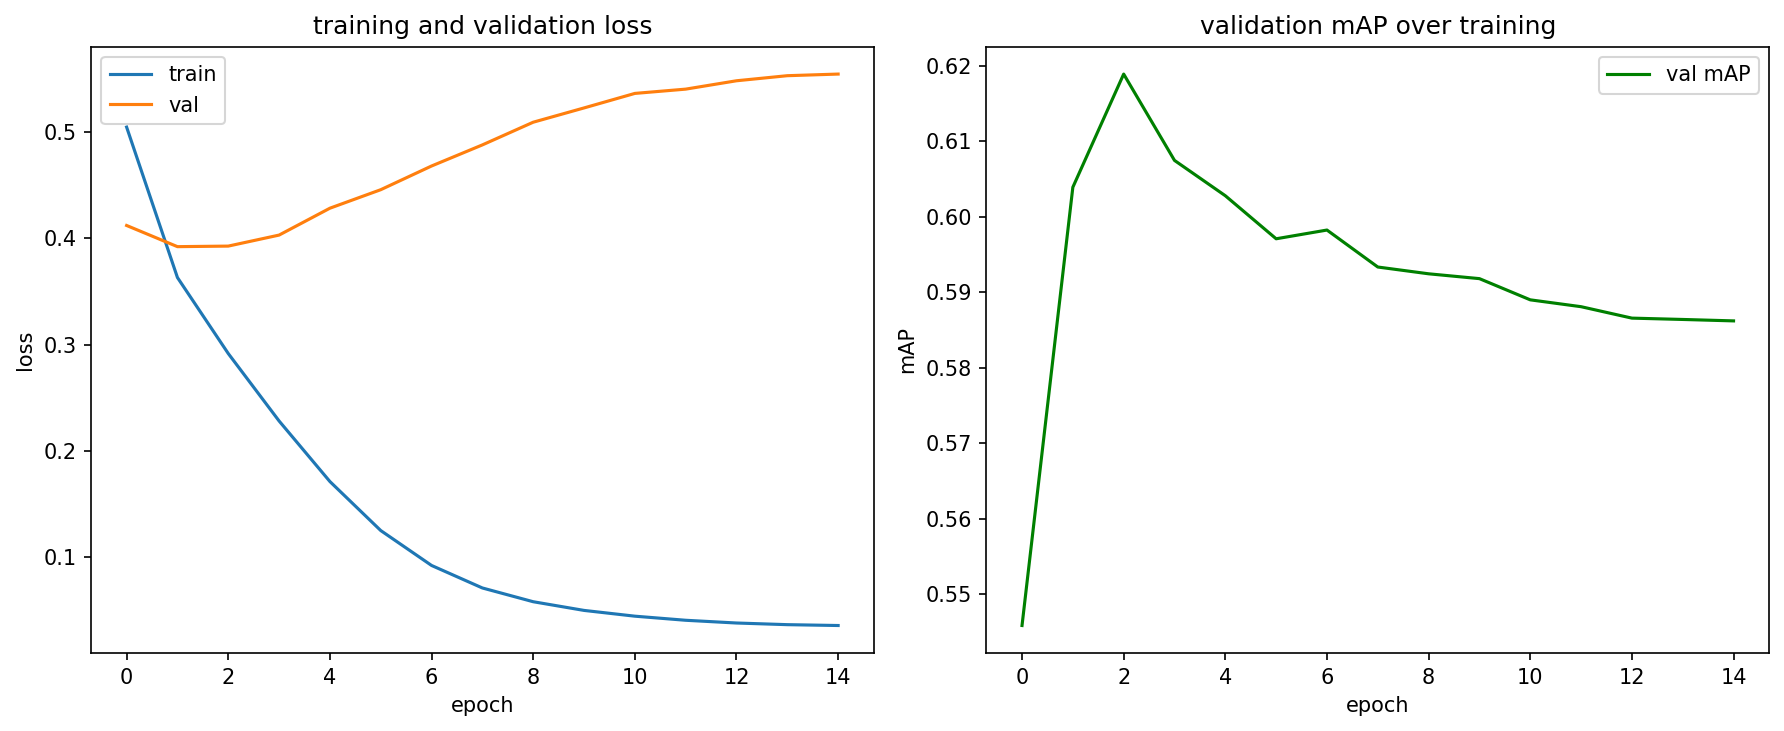
\includegraphics[width=0.9\linewidth]{training_curves_multitask.png}
\end{center}
\begin{itemize}
  \item Best validation loss at epoch 2--3 (mild overfitting after).
  \item Checkpoint selection prevents overfitting from affecting evaluation.
\end{itemize}
\end{frame}

\begin{frame}{Classification Results}
\begin{center}
\begin{tabular}{lc}
\toprule
Method & mAP \\
\midrule
Logistic regression (frozen) & 0.556 \\
MLP classifier (frozen) & 0.566 \\
\midrule
ViT cls-only & 0.623 \\
ViT multitask (KL) & 0.604 \\
\bottomrule
\end{tabular}
\end{center}
\vfill
\begin{itemize}
  \item Fine-tuning improves over frozen baselines by 5--6 mAP points.
  \item Multi-task pays a small cost (1.9 points) vs classification-only.
  \item This is the ``price'' of sharing the backbone with saliency.
\end{itemize}
\end{frame}

\begin{frame}{The MSE vs KL Story}
\begin{center}
\begin{tabular}{lcccc}
\toprule
Saliency Loss & mAP & CC & SIM & KL \\
\midrule
MSE & 0.612 & 0.196 & 0.430 & 1.087 \\
KL divergence & 0.604 & \textbf{0.899} & \textbf{0.799} & \textbf{0.182} \\
\bottomrule
\end{tabular}
\end{center}
\vfill
\begin{itemize}
  \item Same architecture, same data, same optimizer, same $\lambda$.
  \item CC jumps from 0.196 to 0.899 just by switching the loss.
  \item MSE on softmax outputs does not encourage the distribution shape that CC/SIM measure.
  \item KL divergence directly compares probability distributions, aligning the loss with the evaluation metric.
\end{itemize}
\end{frame}

\begin{frame}{Baseline Comparison (Visual)}
\begin{center}
  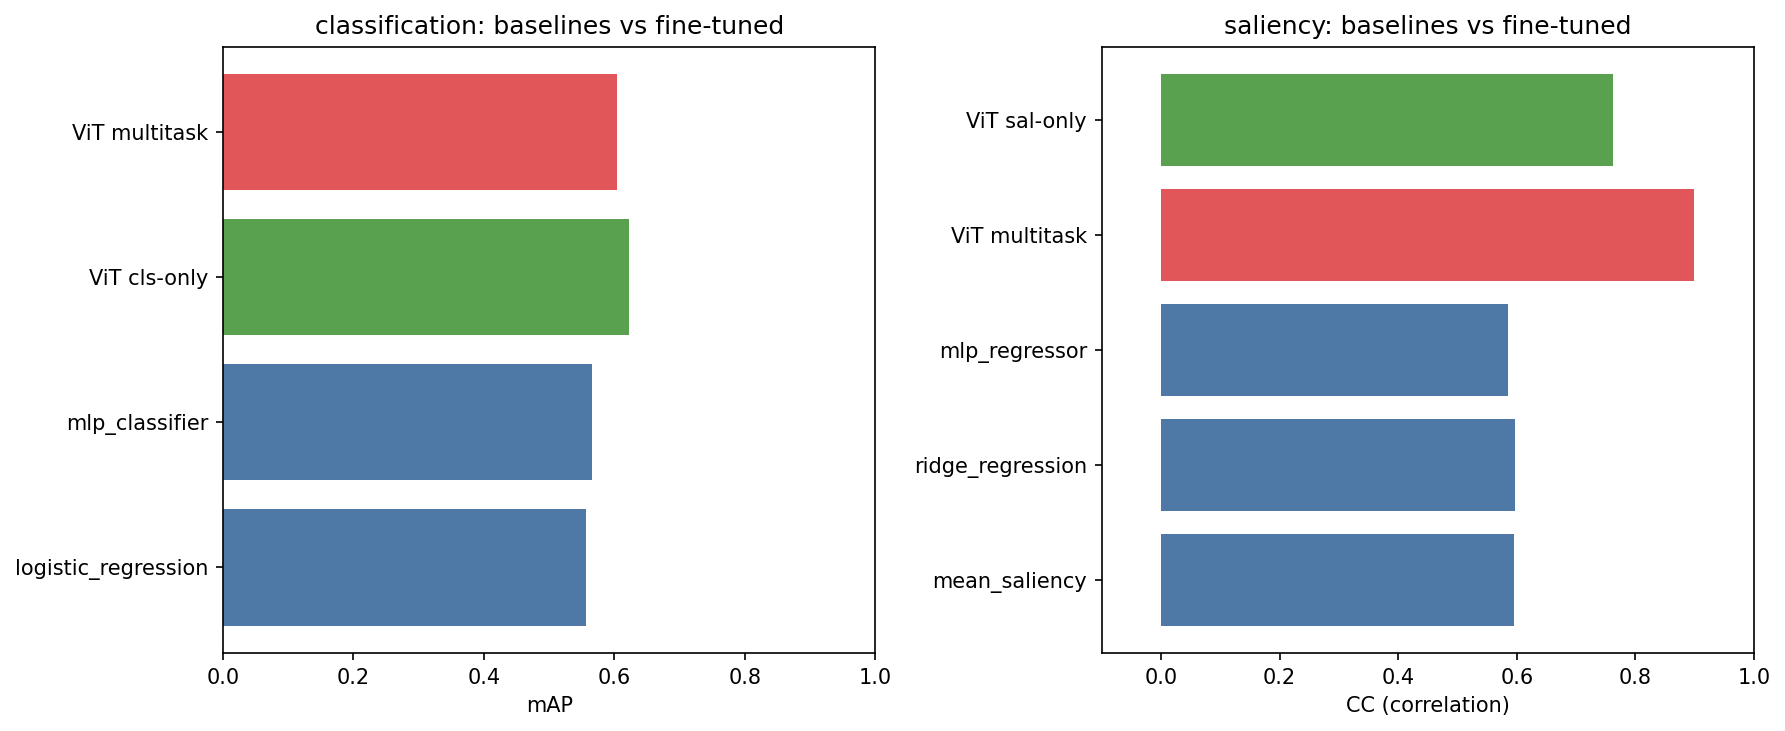
\includegraphics[width=0.9\linewidth]{baseline_comparison.png}
\end{center}
\begin{itemize}
  \item Left: classification mAP. Right: saliency CC.
  \item Fine-tuned models outperform frozen baselines on both tasks.
\end{itemize}
\end{frame}

\begin{frame}{Saliency Prediction Example}
\begin{center}
  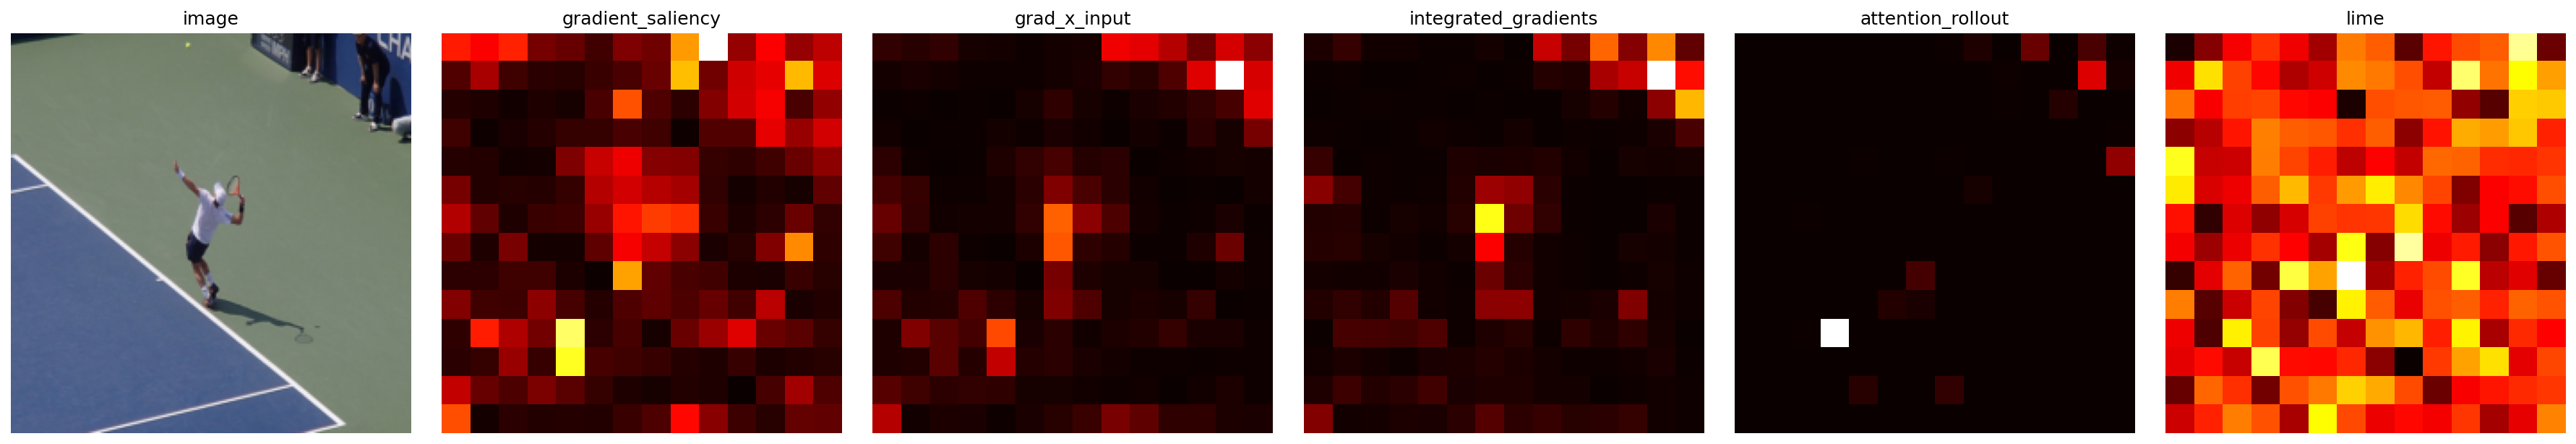
\includegraphics[width=0.85\linewidth]{report_comparison_305.png}
\end{center}
\small A tennis player image. The model's saliency head learns to predict where humans look, concentrating on the player.
\end{frame}

% ============================================================
\section{Conclusion}
% ============================================================

\begin{frame}{Key Takeaways}
\begin{enumerate}
  \item \textbf{Multi-task learning works:} a single ViT can classify and predict saliency simultaneously with modest trade-offs.
  \item \textbf{Fine-tuning beats frozen features:} end-to-end adaptation extracts more task-relevant representations than sklearn baselines on frozen embeddings.
  \item \textbf{Loss design matters:} switching from MSE to KL divergence raises saliency CC from 0.196 to 0.899. Matching the loss to the output parameterization and evaluation metric is critical.
  \item \textbf{Multi-task trade-off is small:} only 1.9 mAP points lost for joint saliency prediction.
\end{enumerate}
\end{frame}

\begin{frame}{Limitations and Future Work}
\begin{itemize}
  \item Single training seed (42); multi-seed runs would strengthen conclusions.
  \item KL and MSE have different gradient magnitudes, so the effective task weighting also shifts; a $\lambda$ sweep would help isolate the loss-alignment effect.
  \item Saliency evaluated at $14 \times 14$ resolution (not comparable to standard SALICON leaderboard scores).
  \item No spatial augmentation; saliency-aware augmentation could help.
  \item Future: $\lambda$ ablation, higher-resolution saliency heads, cross-dataset evaluation.
\end{itemize}
\end{frame}

\begin{frame}
\begin{center}
\Large\textbf{Questions?}

\vfill
\normalsize
Nicholas Welsh \\
\texttt{nwelsh2024@my.fit.edu} \\
\vspace{0.5cm}
Code available upon request.
\end{center}
\end{frame}

\end{document}
